\documentclass[aspectratio=169,11pt]{beamer}

\usepackage[T1]{fontenc}
\usepackage{tgheros}
\usepackage{amsmath}
\usepackage{booktabs}
\usepackage{tikz}
\usepackage{array}

\usefonttheme{professionalfonts}
\renewcommand{\familydefault}{\sfdefault}
\setbeamerfont{title}{series=\bfseries,size=\Large}
\setbeamerfont{frametitle}{series=\bfseries,size=\large}
\setbeamerfont{footline}{size=\scriptsize}

\definecolor{ebdink}{HTML}{1C2834}
\definecolor{ebdgreen}{HTML}{0F6E56}
\definecolor{ebdnavy}{HTML}{1E4D7B}
\definecolor{ebdsage}{HTML}{E7F3EE}
\definecolor{ebdbluepale}{HTML}{E8F0F8}
\definecolor{ebdamber}{HTML}{C56A12}
\definecolor{ebdmuted}{HTML}{5C6B7A}
\definecolor{ebdline}{HTML}{D5DDE3}
\definecolor{ebdtrack}{HTML}{E4E8EC}
\definecolor{ebdwarm}{HTML}{F7F4EC}
\definecolor{ebdcard}{HTML}{FFFFFF}

\setbeamercolor{normal text}{fg=ebdink,bg=ebdwarm}
\setbeamercolor{background canvas}{bg=ebdwarm}
\setbeamercolor{frametitle}{fg=ebdink,bg=ebdwarm}
\setbeamercolor{title}{fg=ebdink}
\setbeamercolor{structure}{fg=ebdgreen}
\setbeamercolor{footline}{fg=ebdmuted,bg=ebdwarm}
\setbeamercolor{itemize item}{fg=ebdgreen}
\setbeamercolor{itemize subitem}{fg=ebdgreen}

\setbeamertemplate{navigation symbols}{}
\setbeamertemplate{itemize item}{\raisebox{0.4ex}{\color{ebdgreen}\rule{1.5mm}{1.5mm}}}
\setbeamertemplate{frametitle}{%
  \vspace{0.35em}%
  {\color{ebdgreen}\scriptsize\insertsection}%
  \par\vspace{0.15em}%
  \insertframetitle\par\vspace{0.15em}%
}
\setbeamertemplate{footline}{%
  \leavevmode\hbox{%
    \begin{beamercolorbox}[wd=0.72\paperwidth,ht=2.6ex,dp=1.1ex,leftskip=1.1em]{footline}%
      \insertdate
    \end{beamercolorbox}%
    \begin{beamercolorbox}[wd=0.28\paperwidth,ht=2.6ex,dp=1.1ex,rightskip=1.1em]{footline}%
      \hfill\insertframenumber\,/\,\inserttotalframenumber
    \end{beamercolorbox}}%
}
\setbeamersize{text margin left=7mm,text margin right=7mm}
\hyphenation{sentence person happen interpretable medical devices}

\newcommand{\hilite}[1]{\textcolor{ebdnavy}{\textit{#1}}}
\newcommand{\card}[3]{%
  \begin{tikzpicture}
    \node[draw=ebdline,fill=ebdcard,rounded corners=2pt,inner sep=7pt,
          text width=#1,align=left,anchor=north west] {#3};
  \end{tikzpicture}%
}
\newcommand{\meter}[2]{%
  \begin{tikzpicture}[baseline=-0.15ex]
    \fill[ebdtrack] (0,0) rectangle (4.6,0.18);
    \fill[#2] (0,0) rectangle ({4.6*(#1)},0.18);
  \end{tikzpicture}%
}

\title{Where the bias sits}
\subtitle{Explainable models, fuzzy rules, and three bias demos}
\author{EBD-AI}
\date{Demos 9--11}
\institute{}

\begin{document}
\setbeamertemplate{footline}{}

\begin{frame}
  \vspace{0.6em}
  {\color{ebdgreen}\scriptsize EBD-AI \textperiodcentered\ DEMOS 9--11}
  \par\vspace{0.7em}
  {\usebeamerfont{title}\Huge Where the bias sits\par}
  \vspace{0.7em}
  {\large First, what an explainable model is.\\[0.25em]
  Then the Titanic, heart-failure, and loan notebooks.}
  \vfill
  {\color{ebdmuted}\small\texttt{ex\_fuzzy} writes the rules.\quad\texttt{ebdai} measures the gaps.}
\end{frame}

\setbeamertemplate{footline}{%
  \leavevmode\hbox{%
    \begin{beamercolorbox}[wd=0.72\paperwidth,ht=2.6ex,dp=1.1ex,leftskip=1.1em]{footline}%
      \insertdate
    \end{beamercolorbox}%
    \begin{beamercolorbox}[wd=0.28\paperwidth,ht=2.6ex,dp=1.1ex,rightskip=1.1em]{footline}%
      \hfill\insertframenumber\,/\,\inserttotalframenumber
    \end{beamercolorbox}}%
}

\begin{frame}
  \vspace{0.35em}
  {\usebeamerfont{frametitle}Thanks\par}
  \vspace{0.15em}
  {\large
  \textbf{Dr Raquel Fern\'andez Peralta}\\[0.2em]
  {\normalsize\color{ebdmuted}UIB, Spain}

  \vspace{0.85em}
  \textbf{Dr Mehrin Kiani}\\[0.2em]
  {\normalsize\color{ebdmuted}Palo Alto Networks, US}

  \vspace{0.85em}
  \textbf{Dr Parastoo Azizinezhad}\\[0.2em]
  {\normalsize\color{ebdmuted}Essex, UK}}
\end{frame}

\section{Foundations}

\begin{frame}{Two parts}
  \begin{columns}[T]
    \begin{column}{0.48\textwidth}
      \colorbox{ebdcard}{\parbox[t]{0.92\textwidth}{%
        {\color{ebdnavy}\large\bfseries 1\quad The model}\\[0.45em]
        Explainable by design\\[0.25em]
        The EU explanation duty\\[0.25em]
        A fuzzy rule classifier}}
    \end{column}
    \begin{column}{0.48\textwidth}
      \colorbox{ebdcard}{\parbox[t]{0.92\textwidth}{%
        {\color{ebdgreen}\large\bfseries 2\quad The bias}\\[0.45em]
        Titanic\\
        the labels already differ\\[0.3em]
        Heart failure\\
        the labels almost agree\\[0.3em]
        Loans\\
        two ways to change the score}}
    \end{column}
  \end{columns}
\end{frame}

\begin{frame}{The model \hilite{is} the explanation}
  \begin{columns}[T]
    \begin{column}{0.48\textwidth}
      \colorbox{ebdcard}{\parbox[t]{0.92\textwidth}{%
        {\color{ebdnavy}\textbf{Post-hoc}}\\[0.4em]
        Train an opaque model.\\
        Afterwards, tell a second story about it.\\[0.45em]
        {\small\color{ebdmuted}That story can disagree with the model that decided.}}}
    \end{column}
    \begin{column}{0.48\textwidth}
      \colorbox{ebdsage}{\parbox[t]{0.92\textwidth}{%
        {\color{ebdgreen}\textbf{By design}}\\[0.4em]
        The decision is already a sentence, plus how strongly it matched this one person.\\[0.45em]
        {\small\texttt{explainable\_predict} returns the class, the winning rule, and the match.}}}
    \end{column}
  \end{columns}
  \vspace{0.7em}
  {\small Readable describes the model. Fair describes the decisions. A rule can avoid the word ``sex'' and still track it through fare, marriage, or income.}
\end{frame}

\begin{frame}{Three things you can read}
  \begin{enumerate}
    \item \textbf{The words.} If sex is used, the word is in the sentence.
    \item \textbf{Who the sentence decides for.} Count how often it wins, inside each group.
    \item \textbf{What the score rewarded.} Demo 11 changes the training score. Watch whether the sentences, the rates, or both move.
  \end{enumerate}
\end{frame}

\section{The rules}

\begin{frame}{Which of this person's data, and how}
  The GDPR asks for meaningful information about the logic of a serious automated decision, and for a way to contest it.
  \vspace{0.55em}

  On 27 February 2025, in a credit-refusal case, the Court of Justice said that means the procedure actually applied: which data were used, and how. Handing over the algorithm is not that explanation.

  \vspace{0.55em}
  \colorbox{ebdsage}{\parbox{0.96\textwidth}{%
    \vspace{0.35em}
    A winning rule \emph{is} that explanation.\\
    ``Refused, because credit history is poor and income is Low.''
    \vspace{0.35em}}}
\end{frame}

\begin{frame}{When those duties apply}
  \small
  \renewcommand{\arraystretch}{1.35}
  \begin{tabular}{@{}l p{0.74\textwidth}@{}}
    \textcolor{ebdnavy}{\textbf{Already}} &
      GDPR explanation, and equal access for women and men to services, including banking. \\
    \textcolor{ebdnavy}{\textbf{2 Aug 2026}} &
      Tell people when they are dealing with an AI system. \\
    \textcolor{ebdnavy}{\textbf{2 Dec 2027}} &
      High-risk duties for credit scoring and other stand-alone uses: outputs a person can interpret, and a check for bias in the data. \\
    \textcolor{ebdnavy}{\textbf{2 Aug 2028}} &
      The same duties when the AI is part of a regulated product, such as many medical devices. \\
  \end{tabular}

  \vspace{0.45em}
  {\scriptsize\color{ebdmuted}Already in force: GDPR Articles 13, 14, 15 and 22, as read in C-203/22, and Directive 2004/113/EC.
  2 August 2026 is Article 50 of the AI Act, Regulation (EU) 2024/1689.
  The later dates are Regulation (EU) 2026/1744. Articles 10, 13, 14 and 86 apply then. This is a map, not legal advice.}
\end{frame}

\section{Fuzzy rules}

\begin{frame}{A hard cutoff flips. A fuzzy word fades.}
  \begin{columns}[T]
    \begin{column}{0.48\textwidth}
      \colorbox{ebdcard}{\parbox[t]{0.92\textwidth}{%
        {\color{ebdnavy}\textbf{Crisp}}\\[0.35em]
        Under 30 is young. One day later, the match goes from 1 to 0.}}
    \end{column}
    \begin{column}{0.48\textwidth}
      \colorbox{ebdsage}{\parbox[t]{0.92\textwidth}{%
        {\color{ebdgreen}\textbf{Fuzzy}}\\[0.35em]
        Membership is anywhere from 0 to 1. One age can be partly Low and partly Medium.}}
    \end{column}
  \end{columns}
  \vspace{0.7em}
  \centering
  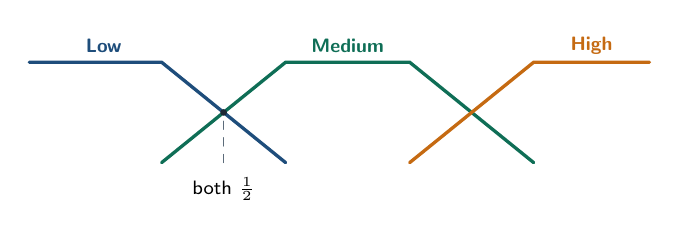
\begin{tikzpicture}[x=1.05cm,y=0.85cm,line cap=round]
    \draw[ebdnavy,very thick] (0.1,1.5) -- (1.7,1.5) -- (3.2,0);
    \node[ebdnavy,font=\scriptsize\bfseries] at (1.0,1.75) {Low};
    \draw[ebdgreen,very thick] (1.7,0) -- (3.2,1.5) -- (4.7,1.5) -- (6.2,0);
    \node[ebdgreen,font=\scriptsize\bfseries] at (3.95,1.75) {Medium};
    \draw[ebdamber,very thick] (4.7,0) -- (6.2,1.5) -- (7.6,1.5);
    \node[ebdamber,font=\scriptsize\bfseries] at (6.9,1.75) {High};
    \draw[ebdmuted,dashed] (2.45,0) -- (2.45,0.75);
    \fill[ebdink] (2.45,0.75) circle (1.2pt);
    \node[font=\scriptsize,anchor=north] at (2.45,-0.08) {both \(\tfrac12\)};
  \end{tikzpicture}

  \vspace{0.35em}
  {\small ``Medium'' is the middle of \emph{this} table. Sex still matches at 1 or at 0.}
\end{frame}

\begin{frame}{The strongest sentence wins}
  Several conditions are \emph{multiplied}. If any one is 0, the rule does not fire.\\
  Sex at 1 and age at one half fires at one half. That product is not yet the decision.
  \vspace{0.4em}

  {\small For one passenger, three rules score as follows. The highest score wins.}
  \vspace{0.55em}

  \renewcommand{\arraystretch}{1.25}
  \begin{tabular}{@{}p{0.72\textwidth} r@{}}
    \toprule
    Rule & Match \\
    \midrule
    Sex is female, and age is Medium & \textcolor{ebdgreen}{\textbf{0.9 wins}} \\
    Age is Low & 0.2 \\
    Fare is High & 0.4 \\
    \bottomrule
  \end{tabular}

  \vspace{0.45em}
  {\small Demos 9 and 10 set every weight to 1, so the match alone decides.\\
  Demo 11 also lets the search choose a weight. A modest match can then win.}
\end{frame}

\begin{frame}{The sentences are searched for}
  \begin{columns}[c]
    \begin{column}{0.32\textwidth}
      \centering
      {\color{ebdnavy}\Huge 12}\\[0.2em]
      {\small candidate rule lists}
    \end{column}
    \begin{column}{0.32\textwidth}
      \centering
      {\color{ebdnavy}\Huge 6}\\[0.2em]
      {\small generations at most}
    \end{column}
    \begin{column}{0.32\textwidth}
      \centering
      {\color{ebdnavy}\Huge MCC}\\[0.2em]
      {\small the score being raised}
    \end{column}
  \end{columns}
  \vspace{0.7em}
  MCC runs from \(-1\) to \(+1\). Accuracy can look fine while the model is lazy, because predicting the common class scores well on an uneven table. The search also stops after 3 generations with no improvement.
  \vspace{0.4em}

  {\small \textbf{DS} is how much a rule carries its own outcome, and how little it fires on the other one. \textbf{ACC} is how often it was right when it won. A rare rule can be 100\% right and still barely matter.}
\end{frame}

\section{The demos}

\begin{frame}{Same questions. Three tables.}
  \small
  \begin{columns}[T]
    \begin{column}{0.32\textwidth}
      \colorbox{ebdcard}{\parbox[t]{0.9\textwidth}{%
        \raggedright
        {\color{ebdnavy}\textbf{9\quad Titanic}}\\[0.3em]
        Labels already differ.\\[0.35em]
        195 of 259 women survive.\\
        93 of 453 men survive.\\[0.3em]
        Test: 49 of 86 women predicted to survive, and no men.\par}}
    \end{column}
    \begin{column}{0.32\textwidth}
      \colorbox{ebdcard}{\parbox[t]{0.9\textwidth}{%
        \raggedright
        {\color{ebdgreen}\textbf{10\quad Heart}}\\[0.3em]
        Labels almost agree.\\[0.35em]
        34 of 105 women die.\\
        62 of 194 men die.\\[0.3em]
        The rule that names sex barely fires.\par}}
    \end{column}
    \begin{column}{0.32\textwidth}
      \colorbox{ebdcard}{\parbox[t]{0.9\textwidth}{%
        \raggedright
        {\color{ebdamber}\textbf{11\quad Loans}}\\[0.3em]
        The score can change.\\[0.35em]
        Label gap about 8 points.\\
        Baseline gap: 30 points.\\[0.3em]
        One repair overshoots. One closes the gap by approving fewer people.\par}}
    \end{column}
  \end{columns}
\end{frame}

\begin{frame}{The label gap, then the prediction gap}
  \begin{columns}[T]
    \begin{column}{0.48\textwidth}
      \colorbox{ebdbluepale}{\parbox[t]{0.92\textwidth}{%
        {\color{ebdnavy}\textbf{In the table}}\\[0.35em]
        How often did the event already occur?\\[0.3em]
        {\small This does not depend on the search.}}}
    \end{column}
    \begin{column}{0.48\textwidth}
      \colorbox{ebdsage}{\parbox[t]{0.92\textwidth}{%
        {\color{ebdgreen}\textbf{In the rules}}\\[0.35em]
        How often is the event predicted, and which sentence won?\\[0.3em]
        {\small This is what the fit did.}}}
    \end{column}
  \end{columns}
  \vspace{0.7em}
  ``Positive'' means the event you chose to count. Survival and approval are benefits. In the heart-failure notebook the event is \textbf{death}.
  \vspace{0.4em}

  {\small A printed gap of \(0.30\) is 30 percentage points. A ratio of 0 usually means one group's rate is zero.}
\end{frame}

\begin{frame}{One group, read four ways}
  Titanic test women: 86 people, 64 of whom survived.
  \vspace{0.4em}

  \renewcommand{\arraystretch}{1.2}
  \begin{tabular}{@{}l l l@{}}
    \toprule
    Count & Name & Meaning \\
    \midrule
    \textbf{49 of 86} & Selection rate & Predicted to survive \\
    \textbf{33 of 64} & True positive rate & Survivors the model caught \\
    \textbf{16 of 22} & False positive rate & Deaths predicted as survival \\
    \textbf{0 of 149} & The other group & Men predicted to survive \\
    \bottomrule
  \end{tabular}

  \vspace{0.45em}
  {\small Equalized odds uses the \emph{larger} of the two error gaps. Here that is 73 points: women who died are often predicted to survive, and men who died never are.}
\end{frame}

\begin{frame}{Titanic: the gap is already in the labels}
  \small
  \begin{tabular}{@{}l c r@{}}
    Women & \meter{0.753}{ebdgreen} & 195 of 259 \\[0.35em]
    Men & \meter{0.205}{ebdnavy} & 93 of 453 \\
  \end{tabular}

  \vspace{0.55em}
  \colorbox{ebdsage}{\parbox{0.96\textwidth}{%
    \vspace{0.3em}
    \textbf{Loudest rule.} If sex is female and age is Medium, then survived.\\[0.25em]
    On the test passengers that rule is the only source of predicted survivals: 49 women, and no men. All 35 men who had survived are predicted to have died.
    \vspace{0.3em}}}
\end{frame}

\begin{frame}{Heart failure: similar labels, one rare rule}
  Death is about one patient in three in both groups.
  \vspace{0.4em}

  \renewcommand{\arraystretch}{1.28}
  \begin{tabular}{@{}r p{0.84\textwidth}@{}}
    \textcolor{ebdgreen}{\textbf{0.54}} & Serum creatinine is Low \quad$\rightarrow$\quad survival \\
    \textcolor{ebdgreen}{\textbf{0.06}} & Ejection fraction is Low \quad$\rightarrow$\quad death \\
    \textcolor{ebdnavy}{\textbf{0.006}} & Anaemia is absent, serum sodium is Medium,\newline and sex is female \quad$\rightarrow$\quad death \\
  \end{tabular}

  \vspace{0.5em}
  The sex rule is right on the few times it wins, and it almost never wins.
  \vspace{0.3em}

  {\small Test predictions of death: 3 of 32 women, 2 of 67 men.}
\end{frame}

\begin{frame}{Loans: the score changes who is approved}
  Test set: 22 women and 137 men. The label gap in the whole table is about 8 points.
  \vspace{0.35em}

  \small
  \renewcommand{\arraystretch}{1.2}
  \begin{tabular}{@{}l c c c c@{}}
    \toprule
     & Women & Men & Gap & Right \\
    \midrule
    Baseline & 6 of 22 & 79 of 137 & 30 pts & 94/159 \\
    Reweighed & 17 of 22 & 45 of 137 & 44 pts, reversed & 83/159 \\
    Penalty & 4 of 22 & 33 of 137 & 6 pts & 68/159 \\
    \bottomrule
  \end{tabular}

  \vspace{0.4em}
  {\small Reweighing makes uncommon group-and-label pairs count more. On this short run it swung past equality.\\
  The penalty is MCC minus \(0.2\) times the gap. The gap closed because both groups were approved less often.}
\end{frame}

\begin{frame}{Four things to write down}
  \begin{enumerate}
    \item The two label counts, \textbf{before} the fit.
    \item Any rule that names the sensitive column, and its DS.
    \item The selection rate as a \textbf{count of people}.
    \item The accuracy beside any new gap.
  \end{enumerate}
  \vfill
  {\small\color{ebdmuted}Numbers are the stored notebook run: one third held out, \texttt{random\_state=42}, at most six generations.}
\end{frame}

\end{document}
